% A simple template for LaTeX documents
% 
% To produce pdf run:
%   $ pdflatex paper.tex 
%


\documentclass[12pt]{article}

% Begin paragraphs with new line
\usepackage{parskip}  

% Change margin size
\usepackage[margin=1in]{geometry}   

% Graphics Example:  (PDF's make for good plots)
\usepackage{graphicx}               
% \centerline{\includegraphics{figure.pdf}}

% subfigures, side by side
\usepackage{subcaption}

% hyperlinks
\usepackage{hyperref}

% Blocks of code
\usepackage{listings}
\lstset{basicstyle=\ttfamily, title=\lstname}
% Insert code like this. replace `plot.R` with file name.
% \lstinputlisting{plot.R}

% Monospaced fonts
%\usepackage{inconsolata}
% GNU \texttt{make} is a nice tool.

% Supports proof environment
\usepackage{amsthm}

% Allows writing \implies and align*
\usepackage{amsmath}

% Allows mathbb{R}
\usepackage{amsfonts}

% Numbers in scientific notation
% \usepackage{siunitx}

% Use tables generated by pandas
\usepackage{booktabs}

% Allows umlaut and non ascii characters
\usepackage[utf8]{inputenc}

% Insert blank pages
\usepackage{afterpage}
%\afterpage{\null\newpage}

% norm and infinity norm
\newcommand{\norm}[1]{\left\lVert#1\right\rVert}
\newcommand{\inorm}[1]{\left\lVert#1\right\rVert_\infty}

% Statistics essentials
\newcommand{\iid}{\text{ iid }}
\newcommand{\Exp}{\operatorname{E}}
\newcommand{\Var}{\operatorname{Var}}
\newcommand{\Cov}{\operatorname{Cov}}


\begin{document}
%%%%%%%%%%%%%%%%%%%%%%%%%%%%%%%%%%%%%%%%%%%%%%%%%%%%%%%%%%%%

The obvious way to make code parallel is to search for the use of
apply functions and transform them into the parallel versions. For example, 
\texttt{lapply()} can be replaced with \texttt{mclapply()} from the
parallel package to use fork based parallelism.

Many of the language idioms in base R already express computation in the
map reduce paradigm.


What to do first:

\begin{itemize}
    \item Is it possibly worth it to parallelize? Software to identify the
        entry points and start with profiling.
    \item SNOW on single node, pure functions
    \item Data abstraction?
\end{itemize}

\subsection{Streaming Parallelism}

This approach resembles the iterators package \cite{R-iterators} which
provides data to R as an abstract stream. The difference is that here
parallelism comes from pipelined operations rather than the more typical
data parallel model.

Let $x$ be a data structure which can be partitioned into chunks $x_1,
\dots x_k$. Chained function calls such as $f(g(h(x)))$ become:

\begin{itemize}
    \item Worker 1: Compute $h(x_i)$, pass result to worker 2
    \item Worker 2: Compute $g(\dots)$, pass result to worker 3
    \item Worker 3: Compute $f(\dots)$.
\end{itemize}

This operation can potentially be efficient if each function $h, g,
f$ takes approximately the same amount of time $T_f$ and $T_f >> T_p$,
where $T_p$ is the time it takes to pipe the data between the 
workers \cite{arnold2015iotools}. More generally, if there is a sequence of
functions $f(x) = f_n(\dots f(_1(x)))$ then a single worker can execute
multiple functions such that the load is balanced. Every added worker will
increase the latency because of communication overhead.


This is a prospectus for distribution to the committee for PhD
Qualifying Exam in June 2017.

\subsection{Pipelines}

This parallel programming pattern is rather different. A useful analogy is a
factory assembly line, with each worker performing one or more operations
and then passing the result to the next worker. The first worker could generate a
subvector of random numbers and pass it along. Ignoring the setup and
looping over chunks the important parts of the code are:

\begin{verbatim}
# Worker 1
x_chunk = rnorm(n_j)
serialize(x_chunk, worker2)
\end{verbatim}

The second worker receives the random numbers and computes the mean.

\begin{verbatim}
# Worker 2
x_chunk = unserialize(worker1)
partial_means[i] = mean(x_chunk)
i = i + 1
\end{verbatim}

This approach is sensible if the load can be balanced across the workers.
Each function should take approximately the same amount of time, and the
overhead required to pass between workers must be much smaller than the
time spent doing work. These assumptions do not all hold in this case,
since if $n = 1000$ then \texttt{xchunk = rnorm(n)} takes 125 $\mu s$,
\texttt{mean(x\_chunk)} takes 6 $\mu s$, and serialization takes at least
15 $\mu s$. On a practical level this can all be implemented over network
sockets or through MPI.


\subsection{Forking}

On a server capable of forking, for example the UC Davis statistics
department servers which have as many as 72 cores, one can use this
approach. Forking uses a \texttt{fork()} system call, which can create
several worker processes with read access to data on the master. This is
efficient if a large data set has been loaded into the manager process.

\begin{verbatim}
x = rnorm(n)

starting_indices = as.integer(seq(from = 1, to = n, by = n_i))
ending_indices = starting_indices + (n_i - 1L)

index_mean = function(start, end) mean(x[start:end])

partial_means = parallel::mcmapply(index_mean, starting_indices, ending_indices)

xbar = mean(partial_means)
\end{verbatim}

This code differs from the SNOW code since each worker can read $x$ without
explicitly exporting it. In statistics we might use this approach for
parallel cross validation of a model, since each worker will need to read
the same data.

\subsection{GPU}

The GPU offers the highest level of parallelism, which could consist of
1000's of threads working at once. Following the OpenCL specification we'll
refer to a GPU as a device, because this can run on other architectures as
well. Here are the simplified steps:

\begin{itemize}
    \item create a kernel which will run in parallel
    \item transfer the data to the device
    \item run the kernel
    \item transfer the results back
\end{itemize}

For this operation the kernel should do the equivalent of the
\texttt{meanrnorm()} function above.  Here's psuedo code for how a kernel
might look in OpenCL, provided the device can fit all of $x$ in memory.
This could be rewritten for larger than device memory by following the
approach in \ref{section:sequential}.

\begin{verbatim}
# include <random.h>

__kernel void meanrnorm(__global float *x
        , __global float *partial_means
        , int n_i
        )
{
    int id = get_global_id(0);

    Random random_state = seed_rand(id);
    int start_index = id * n_i;
    int end_index = start_index + n_i;

    for(int i = start_index; i < end_index; i++)
    {
        random_state = next_rand(random_state);
        x[i] = rnorm(random_state);
    }
    xbar_local = mean(x, start_index, end_index);
    partial_means[id] = xbar_local;
}
\end{verbatim}

This code uses shared memory, since $x$ is a global array.
One can then either write another kernel to reduce
\texttt{partial\_means} on the GPU or return them to the CPU.

\subsection{Threads}

For this problem CPU threads could be utilized in the same way as the GPU.
Indeed, OpenCL was designed to work on multiple platforms including CPU's
and GPU's. The difference is that the memory transfers from host to device
don't take any time, because the host and device are the same.

\subsection{Memory Mapping}

Memory mapping allows one to treat a hard drive as if it is primary memory.
This allows one to have R objects larger than primary memory, and also to
share memory between processes \cite{bigmemory}.

\begin{verbatim}
x = bigmemory::filebacked.big.matrix(nrow = n_i, ncol = p, backingfile = "x.bigmatrix")
for (j in seq(p)){
    x[, j] = rnorm(n_i)
}
xbar = biganalytics::mean(x)
\end{verbatim}

Here \texttt{biganalytics::mean(x)} is used explicitly to emphasize that we
are calling the \texttt{mean()} method defined for \texttt{bigmatrix}
objects.


\section{Code, Data, Platform}
%%%%%%%%%%%%%%%%%%%%%%%%%%%%%%%%%%%%%%%%%%%%%%%%%%%%%%%%%%%%

\textbf{Code} is a script to be executed.
\textbf{Data} could be data in memory, single or multiple files, a
memory-mapped file, a database, a parallel file system, etc.
\textbf{Platform} is the computing setup, such as a laptop with 4 cores, a
Spark cluster, or a server with 2 GPUs and a high bandwidth connection. The combination
of (Code, Data, Platform) dictates what strategies should be used for
efficient evaluation. Given these three components, our goal is to analyze the
code, potentially reorganizing it for efficient execution on the data and
platform. This doesn't mean that the system is inventing new algorithms on
the fly. But it should be capable of tuning existing parameters to the
system at hand. An example of a parameter to be tuned is the chunk size
$n_i$ as described in \ref{section:sequential}.

This project is in the spirit of compiling R, since it treats R code as
a set of high level directions, and it potentially generates alternative
code for execution \cite{lang2014enhancing}.

\section{Motivating Example}
%%%%%%%%%%%%%%%%%%%%%%%%%%%%%%%%%%%%%%%%%%%%%%%%%%%%%%%%%%%%
\label{sec:pems}

The California Department of Transportation collects traffic data through
sensors embedded in highways. The sensors measure three quantities: count
of passing vehicles, time during which a vehicle is directly above the
sensor (occupancy), and average velocity \cite{jia2001pems}.  Every thirty
seconds they produce a new data point. $43,680$ sensors in California
measuring 3 parameters multiplied by $(2 \times 60 \times 24)$ measurements
per day results in 377 million new data points per day.  This raw data is
organized into files grouped by (day, district), and is available for
public download.  As an analyst I would like to model velocity as a
function of occupancy for each sensor. This relationship is called the
``fundamental diagram'' within traffic engineering, because it captures the
operating characteristic of this section of road
\cite{daganzo1997fundamentals}. Once these fundamental diagrams have been
modeled for each station they can be used to understand how other road
characteristics such as on ramps and off ramps affect the flow of traffic.

Robust regression can be used to fit the fundamental diagram, approximating
the integer programming approach to minimize the L1 norm as in
\cite{li2011fundamental}.  From the R language this can be done easily and
efficiently, for example with the \texttt{rlm} (robust linear model)
function in the MASS package \cite{venables2013modern}:

\begin{verbatim}
fit1 = rlm(velocity ~ occupancy, data = station1)
\end{verbatim}

However, the size and organization of the data makes the task much more
difficult.  I've downloaded a subset of the data consisting of measurements
in the San Francisco Bay Area for part of 2016.  It would be easier to
perform the regression if the data were organized in files for each sensor
rather than in files for each day.  One approach then is to reorganize the
data on disk into this file structure. I did this using a simple single
threaded R program, and it took 23 hours to run on 134 GB of data.
Throughput for a conventional hard disk is around 100 MB/s\footnote{RAID,
an array of disks, could make this faster.}, so a lower bound for reading
then writing this reorganized data is approximately $2 * 134000 / 100$
seconds, or 45 minutes. The naive code is 30 times slower than this. So
small inefficiencies add up.

Another drawback is that it requires very specific instructions to
reorganize the data for computations grouped by station. Any parallel
programming will make this even more specific to the data and platform. The
following R code captures the desired semantics:

\begin{verbatim}
by(data, INDICES = station, FUN = piecewise_rlm)
\end{verbatim}

This says group \texttt{data} by \texttt{station}, and apply the
function \texttt{piecewise\_rlm} to each group.

What if we had a system that could inspect the idiomatic R code above that
works on small data sets, and then automatically take steps to scale and to
parallelize the operations? It could also tune them for the specifics of
the system and the data. This is what we're working towards.


\section{Simple Example}
%%%%%%%%%%%%%%%%%%%%%%%%%%%%%%%%%%%%%%%%%%%%%%%%%%%%%%%%%%%%

% Duncan:
% Come up with concrete and realistic examples.  Show how you would do things
% differently for different computational platform Go through this explicitly
% by hand to show the "ideal" transformed code (keep high level) Identify how
% you might identify these programmatically and what are some of the
% challenges

Now we use a simple example to focus on the underlying computational models
for various platforms.  Consider computing the mean,

\begin{equation}
    \bar{x} = \frac{1}{n} \sum_{i = 1}^n x_i
\label{eq:mean}
\end{equation}

where the $x_i$'s are
i.i.d. $\sim N(0, 1)$.  In R this code is written:

\begin{verbatim}
xbar = mean(rnorm(n))
\end{verbatim}

To evaluate this R will first build an intermediate vector $x = (x_1,
\dots, x_n)$ and then compute the mean. Eventually that unreferenced
intermediate vector will be garbage collected.
Execution time increases
linearly with $n$. Once $n$ becomes large
enough this vector will no longer fit into available physical memory, so
the operating system will use swap space. On a machine with 8 GB memory
this happens when $O(n) = 10^9$, causing the execution time
to increase by an order of magnitude, roughly from 1 minute to 15
minutes. Once $n$ exceeds memory and swap space R will not be able to allocate a
large enough object, and the computation will fail.

Now we consider alternative ways to execute this code.  Most rely on
splitting the sum into $p$ partial sums with $n_j$ terms each and then rewriting
Equation \ref{eq:mean} as a weighted mean.

\begin{equation}
    \bar{x} = \frac{1}{n} \sum_{j = 1}^p \sum_{i = 1}^{n_j} x_{ij}
    = \sum_{j = 1}^p \frac{n_j}{n} \bar{x}_j
\label{eq:mean_partial}
\end{equation}

It's important to correctly handle the cases when $n$ is not divisible by $p$
and the computation / data cannot be evenly split. For simplicity in the
examples below, suppose that they can be split evenly so $n_i$ is the same
for all $i$.

\subsection{Sequential Execution}
\label{section:sequential}

Equation \ref{eq:mean_partial} can be directly translated into R code as
follows:

\begin{verbatim}

n = 1e5
p = 10
n_i = as.integer(n / p)

meanrnorm = function(n) mean(rnorm(n))

partial_means = sapply(rep(n_i, p), meanrnorm)
xbar = mean(partial_means)
\end{verbatim}

This code does not run in parallel, but it does use the same functional
programming patterns as parallel code. If $M$ is the size of physical memory in
bytes then this code is high performance in the sense
that execution time will continue to be linear while $n < O(M^2)$, just
as it was for small $n < O(M)$. It can also be modified to handle
arbitrarily large $n$. This is because \texttt{sapply} runs
sequentially, so the memory footprint can be bounded since the intermediate
vectors will be of length $n / p$. 

What aspects of the code changed? In the initial code the user
supplied $n$, and it remained to choose $p$ and $n_i$.
The expression \texttt{mean(rnorm(n))} was changed into a function that was
called and reduced using \texttt{mean()}.

\subsection{SNOW Cluster}

Clusters created by SNOW, a Simple Network Of Workstations,
consist of independent worker R processes created by a manager process. The
processes communicate over network sockets, and they may be on one or many
physical machines.  This is the type of cluster used by partools and
Software Alchemy \cite{R-partools} \cite{matloff2014software}.  This is
similar to \ref{section:sequential}; the \texttt{sapply}
becomes:

\begin{verbatim}
partial_means = parallel::clusterCall(cluster, meanrnorm, n_i)
\end{verbatim}

The manager sends the \texttt{meanrnorm()} function to each worker in the
cluster to be evaluated in parallel with argument \texttt{n\_i}.  Given an
existing cluster this is very efficient, since we are sending a few bytes
of code over the network and then returning a single number. This parallel model is
useful in statistics when doing independent simulations.

\subsection{Forking}

On a server capable of forking, for example the UC Davis statistics
department servers which have as many as 72 cores, one can use this
approach. Forking uses a \texttt{fork()} system call, which can create
several worker processes with read access to data on the master. This is
efficient if a large data set has been loaded into the manager process.

\begin{verbatim}
x = rnorm(n)

starting_indices = as.integer(seq(from = 1, to = n, by = n_i))
ending_indices = starting_indices + (n_i - 1L)

index_mean = function(start, end) mean(x[start:end])

partial_means = parallel::mcmapply(index_mean, starting_indices, ending_indices)

xbar = mean(partial_means)
\end{verbatim}

This code differs from the SNOW code since each worker can read $x$ without
explicitly exporting it. In statistics we might use this approach for
parallel cross validation of a model, since each worker will need to read
the same data.

\subsection{GPU}

The GPU offers the highest level of parallelism, which could consist of
1000's of threads working at once. Following the OpenCL specification we'll
refer to a GPU as a device, because this can run on other architectures as
well. Here are the simplified steps:

\begin{itemize}
    \item create a kernel which will run in parallel
    \item transfer the data to the device
    \item run the kernel
    \item transfer the results back
\end{itemize}

For this operation the kernel should do the equivalent of the
\texttt{meanrnorm()} function above.  Here's psuedo code for how a kernel
might look in OpenCL, provided the device can fit all of $x$ in memory.
This could be rewritten for larger than device memory by following the
approach in \ref{section:sequential}.

\begin{verbatim}
# include <random.h>

__kernel void meanrnorm(__global float *x
        , __global float *partial_means
        , int n_i
        )
{
    int id = get_global_id(0);

    Random random_state = seed_rand(id);
    int start_index = id * n_i;
    int end_index = start_index + n_i;

    for(int i = start_index; i < end_index; i++)
    {
        random_state = next_rand(random_state);
        x[i] = rnorm(random_state);
    }
    xbar_local = mean(x, start_index, end_index);
    partial_means[id] = xbar_local;
}
\end{verbatim}

This code uses shared memory, since $x$ is a global array.
One can then either write another kernel to reduce
\texttt{partial\_means} on the GPU or return them to the CPU.

\subsection{Threads}

For this problem CPU threads could be utilized in the same way as the GPU.
Indeed, OpenCL was designed to work on multiple platforms including CPU's
and GPU's. The difference is that the memory transfers from host to device
don't take any time, because the host and device are the same.

\subsection{Memory Mapping}

Memory mapping allows one to treat a hard drive as if it is primary memory.
This allows one to have R objects larger than primary memory, and also to
share memory between processes \cite{bigmemory}.

\begin{verbatim}
x = bigmemory::filebacked.big.matrix(nrow = n_i, ncol = p, backingfile = "x.bigmatrix")
for (j in seq(p)){
    x[, j] = rnorm(n_i)
}
xbar = biganalytics::mean(x)
\end{verbatim}

Here \texttt{biganalytics::mean(x)} is used explicitly to emphasize that we
are calling the \texttt{mean()} method defined for \texttt{bigmatrix}
objects.

\subsection{Pipelines}

This parallel programming pattern is rather different. A useful analogy is a
factory assembly line, with each worker performing one or more operations
and then passing the result to the next worker. The first worker could generate a
subvector of random numbers and pass it along. Ignoring the setup and
looping over chunks the important parts of the code are:

\begin{verbatim}
# Worker 1
x_chunk = rnorm(n_i)
serialize(x_chunk, worker2)
\end{verbatim}

The second worker receives the random numbers and computes the mean.

\begin{verbatim}
# Worker 2
x_chunk = unserialize(worker1)
partial_means[i] = mean(x_chunk)
i = i + 1
\end{verbatim}

This approach is sensible if the load can be balanced across the workers.
Each function should take approximately the same amount of time, and the
overhead required to pass between workers must be much smaller than the
time spent doing work. These assumptions do not all hold in this case,
since if $n = 1000$ then \texttt{xchunk = rnorm(n)} takes 125 $\mu s$,
\texttt{mean(x\_chunk)} takes 6 $\mu s$, and serialization takes at least
15 $\mu s$. On a practical level this can all be implemented over network
sockets or through MPI.

\section{Design Considerations}
%%%%%%%%%%%%%%%%%%%%%%%%%%%%%%%%%%%%%%%%%%%%%%%%%%%%%%%%%%%%

The approaches in the previous section can sometimes be combined together
into hybrid approaches. For example, forked process might run multithreaded
code.

\subsection{Overhead}

Many of the performance characteristics of the different platforms can be
understood in terms of the overhead to set them up, and then the latency
and bandwidth for when data must be transferred.  If the data is ``small
enough'' then performance will be acceptable regardless of how well the
platform is utilized or how efficient the code is. Conversely, if the data
is ``large enough'' then \emph{everything} matters, since small
inefficiencies will be magnified when they occur millions of times, as in
Section \ref{sec:pems}.  Therefore the focus here is on problems which take longer
to run. A priori one doesn't even know if it's possible to run code more
efficiently in parallel, due to the overhead.

\begin{figure}
\centering
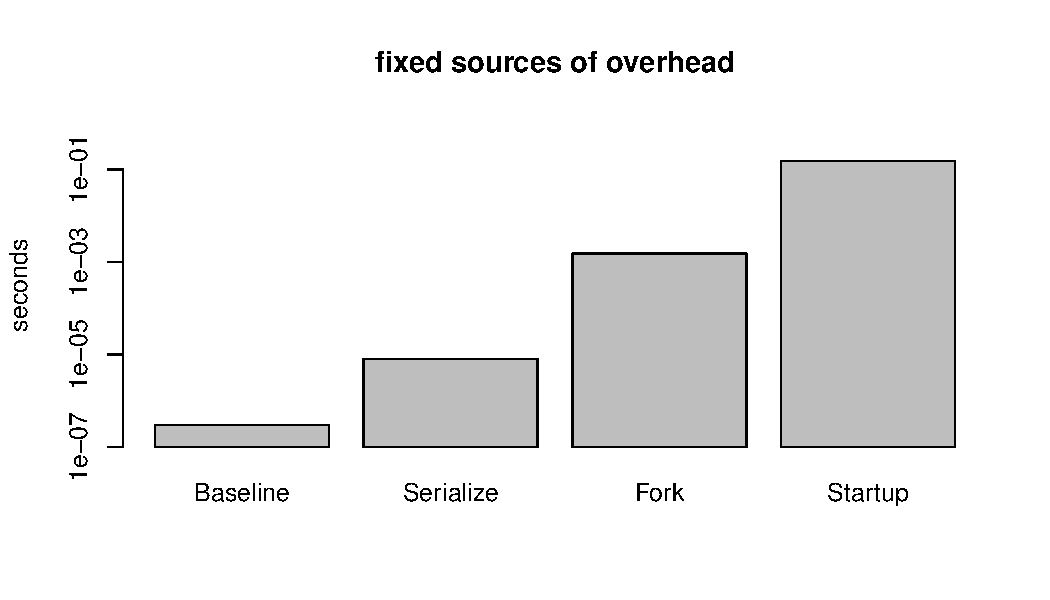
\includegraphics[width=.8\linewidth]{compute_times/overhead}
\caption{Simple function calls take less than a microsecond. Launching a
    new R interpreter takes hundreds of milliseconds, which is relatively expensive.}
\label{fig:overhead}
\end{figure}

Figure \ref{fig:overhead} compares the relative fixed sources of overhead to
consider with parallel programming. The evaluation of the following simple
function captures the basic overhead associated with an interpreted
language like R:
\begin{verbatim}
twox = function(x) 2*x
\end{verbatim}
Every call to this function will incur a fixed overhead that is a couple
hundred nanoseconds. Vectorization refers to passing longer vectors to the
function to amortize this fixed cost. For example, if $x$ is an integer
vector of length 1 then the overhead takes 2 orders of magnitude more time
than the actual computation. However, if $x$ is of length 1500 then this
overhead accounts for only 10 percent of the total execution time, so the
fixed cost has been amortized.

\subsection{Interfaces}

Parallel programming in pure R (not at the C level) can be understood in
terms of a layered architecture. The foundational \textbf{System Layer}
provides the basic interfaces used by any programming language. The
\textbf{R Layer} consists of packages which adapt the basic interfaces for
use specifically in R. The packages in the \textbf{User Layer} are meant to
simplify parallel programming, or they are for applications with specific
use cases.  Here are a few examples of packages at each layer:

\begin{itemize}
\item User Layer: foreach, future, partools, ddR, biganalytics, RevoScaleR
\item R layer: SNOW, multicore, parallel, bigmemory, Rmpi
\item System Layer: processes, *NIX fork(), memory maps, network sockets,
    MPI
\end{itemize}

Currently, users write code using packages from the User Layer or the R
Layer. Code analysis potentially can allow us to skip these layers, and
instead write the same base R code which will run in serial as in parallel.
This is appealing for a few reasons. Base R is stable, so users can write
the same working code without committing to a particular package or
architecture. If the code runs on a different system or with a different
data set then one can automatically generate code to run more efficiently
on that system.

%TODO: expand
Some of the work here may mean enhancing the capabilities of these
intermediate layers. For example, a file based sort usable from R allows
``group by'' and facilitiates streaming applications.

\section{Code analysis}
%%%%%%%%%%%%%%%%%%%%%%%%%%%%%%%%%%%%%%%%%%%%%%%%%%%%%%%%%%%%

Static code analysis is integral to this approach, and we build on the 
CodeDepends package \cite{R-CodeDepends}.

\subsection{Streaming Parallelism}

This approach resembles the iterators package \cite{R-iterators} which
provides data to R as an abstract stream. The difference is that here
parallelism comes from pipelined operations rather than the more typical
data parallel model.

Let $x$ be a data structure which can be partitioned into chunks $x_1,
\dots x_k$. Chained function calls such as $f(g(h(x)))$ become:

\begin{itemize}
    \item Worker 1: Compute $h(x_i)$, pass result to worker 2
    \item Worker 2: Compute $g(\dots)$, pass result to worker 3
    \item Worker 3: Compute $f(\dots)$.
\end{itemize}

This operation can potentially be efficient if each function $h, g,
f$ takes approximately the same amount of time $T_f$ and $T_f >> T_p$,
where $T_p$ is the time it takes to pipe the data between the 
workers \cite{arnold2015iotools}. More generally, if there is a sequence of
functions $f(x) = f_n(\dots f(_1(x)))$ then a single worker can execute
multiple functions such that the load is balanced. Every added worker will
increase the latency because of communication overhead.

\subsection{Apply functions}

The obvious way to make code parallel is to search for the use of
apply functions and transform them into the parallel versions. For example, 
\texttt{lapply()} can be replaced with \texttt{mclapply()} from the
parallel package to use fork based parallelism.

Many of the language idioms in base R already express computation in the
map reduce paradigm.

\subsection{Vectorization}

Vectorization

Goes hand in hand with loop fusion.


\subsection{Reduce functions}

\texttt{mean()} as used in \texttt{mean(rnorm(n))} reduces a vector to a
single number. Here's one way to write this using \texttt{Map(), Reduce()}
explicitly in R:

\begin{verbatim}

N = 100
p = 9
weightmean = function(x_i, N) (length(x_i) / N) * mean(x_i)

x = rnorm(N)
xsplit = split(x, seq(p))
parts = Map(weightmean, xsplit, N = N)
xbar1 = Reduce(`+`, parts, 0)

# matches up to numerical precision
xbar2 = mean(x)

\end{verbatim}

\subsection{Optimization problem}

One way to approach the question of how to run the code is as an
optimization problem. The objective function to minimize is the total run
time. The solution needs to select an appropriate computational model. Each
model may have various parameters to optimize over, for example:

\begin{itemize}
    \item number of processor cores to use
    \item size of each chunk
    \item which functions to combine in one processing step
\end{itemize}

Constraints may include:

\begin{itemize}
    \item number of cores available
    \item network bandwidth
    \item disk IO speed
    \item available memory
\end{itemize}

\subsection{Statistical Problem}

The time it takes for the same computations to execute can vary quite a
bit. Let $x_i$ be a data vector of length $n_i$. Suppose we want to evaluate
$f(x_i)$ in parallel.

Consider these parameters:

\begin{itemize}
    \item $w$ time to start up a worker process
    \item $l$ latency for communication between manager and worker
    \item $t(n_i)$ time required to compute $f(x_i)$ on the worker
\end{itemize}

Then starting without a cluster it takes
\[
    T_i = w + 2l + t(n_i)
\]
to evaluate an expression on a worker. If the worker already exists then
take $w = 0$.

\subsection{Dependency Analysis}


\section{Databases}

What if we could \texttt{attach()} the tables from a database into R? Then users
could write code as if the data were in R. We could figure out the chunking
based on their code.


\subsection{Data Movement}
%%%%%%%%%%%%%%%%%%%%%%%%%%%%%%%%%%%%%%%%%%%%%%%%%%%%%%%%%%%%

Moving data is slow and therefore should be minimized. It can be slow in
terms of latency and also because of bandwidth. Examples of this include
transferring data over a network, where latency can be measured in
milliseconds and bandwidth in MB per second.

Initially assume that the code is correct. Consider an example of code that
reads a file, performs a computation, and saves the result in a file.
Most approaches to improving performance or scaling to large datasets
come from \emph{manually rewriting} the code, tailoring it to this
particular application. It's better to avoid this if possible.  Code that's
rewritten for performance results in an increase in complexity
\cite{matloff2015parallel}.  Compilation is one way to keep the original
code and get more speed. Translation and metaprogramming are another way.
Translation here refers to taking the code and modifying it, for example by
adding statements.


\section{Approximating data size}
%%%%%%%%%%%%%%%%%%%%%%%%%%%%%%%%%%%%%%%%%%%%%%%%%%%%%%%%%%%%

For data in files one could read the first several records along with the
data size and make an inference as to how many rows there are, and come up
with an appropriate evaluation scheme. This is similar to how column
inferences work.

\section{Introduction}
%%%%%%%%%%%%%%%%%%%%%%%%%%%%%%%%%%%%%%%%%%%%%%%%%%%%%%%%%%%%

What new things am I bringing to the table? My QE is in two months, time to
focus.

General idea- code analysis to detect and use parallelism. Determining and
using a chunking scheme based on (code, platform, data).

Running without chunks is the same as regular vectorized R- one can think
of this as a degenerate case of chunked operations with just one chunk.

Broad idea- more separation between the high level language
and the implementation. This is consistent with the idea of R as a `wrapper'
language, providing a convenient interface for numerical routines written
in a faster language \cite{chambers2016extending}.

Right now seems like a very good time to be pursuing this, since many of the
building blocks are in place:
\begin{itemize}
    \item Fast IO packages
    \item SNOW and parallel
\end{itemize}

partools in particular is a nice base to build on.

One could think about this as a system architecturally organized in layers- building on
partools, say, which builds on SNOW. Users are free to enter at any layer.

Idea for metadata- see notes in partools. Could use a data structure
describing characteristics for how each chunk of the data is accessed,
ideally along with something about the sizes. Something like a schema.
Code analysis seems like the most esoteric thing compared to the others.

Some functions can be applied in a streaming manner, where they visit the
data. Can we detect these functions programmatically? If we can then this
gives free parallelism.

I'd like to examine the code and determine where parallelism will give the
most benefit. Ie. nesting parallelism will likely hurt. But how much? And
can we detect it?

TODO: check. This is consistent with results \cite{chambers2016extending}


I believe that similar ideas hold for compiled languages. The overhead will
be different, generally much less. And threads can be used for handing off
and directly manipulating the same objects.

\section{Chunking Approaches to Large Data}
%%%%%%%%%%%%%%%%%%%%%%%%%%%%%%%%%%%%%%%%%%%%%%%%%%%%%%%%%%%%

To stay in memory we use chunked computations. If the chunks are too small
they'll be inefficient. Then how do we choose the chunk size?  There may be
a ``sweet spot'' or range of values for computation as well as for
statistical accuracy. For example, for software alchemy to work it's
necessary that the chunk sizes increase towards infinity
\cite{matloff2014software}.



\textbf{Speculative evaluation of different chunked computation schemes}

A well known technique for parallel computation is to split data into
chunks and compute on each chunk simultaneously. This approach 
is useful on large data. Multiplying large block matrices is an example of this.

Many existing software packages for parallel computation requires one to specify the
chunk size. Examples include ddR \cite{R-ddR} and partools
\cite{R-partools} in R and dask in Python.
Yet chunk size strongly impacts
performance. If it's too small then there will be excessive overhead. If
it's too large then it won't fit into memory. In both cases performance
will suffer. But how much will it suffer?

Matloff presents compelling reasons to use a chunk based
approach for statistical applications \cite{matloff2014software}.

\subsection{Related Work}

Python's dask library infers appropriate block size for
\href{https://github.com/dask/dask/pull/1328}{reading CSV files}.

R's bigmemory package uses C++ and a memory mapped file which allows shared
memory access. \cite{kane2010bigmemory} It's a tool for representing large
data sets, and the package vignette mentions that chunking can and should
be used together when possible.

\subsection{Challenges}

For a given set of hardware and a given task graph in a given
computational model there may be
an optimal chunking scheme, or a range of chunk sizes with similar performance.
We'd like to automatically figure that out so the user doesn't have to
specify. It may be possible to gather data be speculatively running parts
of the computation and then using this as the inputs to a 
mathematical optimization problem.

I'd expect that a dynamic language calling vectorized C code has some set
of performance characteristics, while standalone C++ code is quite
different.
Extension: What chunking is optimal for GPU?

Allowing \texttt{rechunk()} operations in the middle of the task graph adds
much more flexibility and complexity. But it might be useful.

Need to be a little careful because the chunking scheme defines the dask
task graph. Then the semantics are more general than the dask graph. It's
really similar to optimization.

\subsection{Applications}

Google's TensorFlow can express large computational graphs on n dimensional
arrays (tensors), mostly for machine learning.

Apache Spark does chunking transparently to the user, and it's possible to
tune it for performance reasons.


\section{Chunking}

IDEA: nested parallelism- how to do it? If you hard code it in you're
stuck.

The task based parallelism isn't as relevant to how people use R (and other
languages) for data processing. Instead
lets think more about chunking and data parallelism. 

Parallelism introduces additional overhead on top of what dynamic languages
already incur. A general strategy to minimize this overhead is to ``chunk''
the computations. For example, given 1000 parallel operations one might
partition these into chunks of size 100 so that they become 10 parallel
tasks \cite{matloff2015parallel}.

I can take the code in \cite{matloff2015parallel} and see how changing the
chunk sizes affects the run time. I could also do this with Python's dask.
The goal is to draw general conclusions about which chunk sizes work best
based on the amount of computation.

It would be nice to run just a couple in serial on the master process and
make principled decisions about how to run based on these results. For
example:
\begin{itemize}
    \item Is it worth it to run in parallel?
    \item Should we chunk? What should the chunk sizes be?
    \item Reverse the order for better load balancing?
    \item Dynamic or static scheduling?
\end{itemize}

Usually none of these are known ahead of time.  They also depend on the
particular problem.  The only way to know if a chunking scheme will work is
to experiment with a similar problem, then check expectations for the next
one. I also expect that they vary across different machines.

The book mentions using large chunks in the beginning followed by small
chunks for superior load balancing.

Programming in the RDSM package conceptually is very similar to OpenCL on
the GPU. You allocate memory and send it to the workers, then update it in
place based on thread IDs. This is quite different than normal functional
R. I wonder if we could "translate" regular R into this style of
programming?

TODO: Come up with application where I need all this!! How about computing
graphs from Euclidean space like with James' application? It would be nice
for the QE to have something that he's familiar with and invested in.

\section{Software Alchemy}

Looking at Norm's book now. He mentions tuning Software Alchemy for
statistical purposes through chunk size. But I've been thinking about just
tuning them for computational efficiency. Perhaps these two different
lenses could be combined?

\section{Applications}

Goal: Fit a piecwise linear fundamental diagram for each station ID using
30 second data, following \cite{li2011fundamental}. Preprocess the
observations to remove obviously bad data points.  Fit using robust
regression to limit the effect of outliers.  

Each file is around 1 GB when loaded in R, and there are several hundred
files (we could actually take as many as we like). So this is beyond the
limits of what we can do in memory even on a server.

This is all done to reduce the data for one station into several summary
statistics. The main summary statistic of interest is the piecewise linear
fundamental diagram. This may be different for different weather patterns. 
Goodness of fit statistics for each station / fundamental diagram are
important because they indicate places where a piecewise linear fit may
have been inadequate, or the data had excessive noise.

These fundamental diagrams and related statistics can then be used to
classify and distinguish between the stations. For example, the right hand
lane has more trucks and therefore one can expect a different kind of
fundamental diagram. It's expected that the shape and parameters of the
fundamental diagram relate to the locations of on ramps and off ramps
relative to the stations. To precisely quantify these things we need to
compute the statistics. On a broader note, these inferences can be used for
better transportation planning.

This can't be easily done in a database because robust regression is
a relatively specialized method, yet available in MASS::rlm.
Ideally we could combine the best of both worlds.

This is difficult because the data files are split by day, yet we
need to group by station ID, which shows up in every day.

Now I'm thinking about how to do this split. The ff package looks
appealing, but unmaintained for a little while. iotools and data.table
are also appealing to get high performance read / write. Let's see if I
can do this split with iotools pipeline parallelism

I could perform a file based split in several ways- with Spark, dask, and
rolling my own in R. I suspect that dask or R will be the easiest.

R- Advantage is that one can stay in the same system as where the analysis
will be done. 

Dask- Probably performs well

Spark- Putting the data into the SQL database would be pretty nice for
future work.

First I should do it one way. Let's go with R since I've already started.
I did the file based split with base R, no parallelism and it took 1402 minutes = 23.4 hours.

Big Data:

Norm was talking about the buzz around Hadoop mostly being a lot of hype.
Simon Urbanek processes crazy amounts of data using just plain old R.

\emph{While “Big Data” tools can be exciting, they are almost always worse than
normal data tools while those remain appropriate.} - Dask documentation

One problem is that moving to an entirely different system can require
completely rethinking your approach. dplyr and sparklyr are appealing in this
aspect because they basically use the same user API and do the right
thing at the backend. As with SQL, they're also more high level / descriptive of the
desired operation. Then we have this tension between simple code and
complex code. The simple code is easier to maintain and understand, while
the complex code is adapted to the system / problem at hand. A high level
idea is to take the simple code and make it perform as well or better than
the complex code necessary to run it in a more sophisticated way- ie. on a
parallel machine or a GPU.

In general one doesn't want to think about the chunks. At all.

A personal frustration I've experienced with the database type R interfaces
is that it's not possible to directly write user defined R that will work.
Most R / database interfaces that I've seen essentially allow one to do the
same thing in R as one could do in SQL. This is not helpful for me, because
I could just write the SQL myself. I use R not because I love the syntax,
rather I want the convenient and correct statistical functionality.

\section{Streams}

Thinking about the streaming example. Can we look at a
piece of code and determine if it can be converted to a streaming function?
This can be done for functions that are vectorized, ie. they compute things
elementwise. It can be done for functions that use a for loop over the
indices. 

It can't be done for more complex operations like sorting.

How about for compositions of streaming functions? Sure, this amounts to
loop fusion.

Reducing

\section{Examples}

Consider making a prediction vector for some $n \times p$ matrix $X$. In
the conventional case the prediction for each row is independent so this is
embarrassingly parallel.\footnote{More generally, with something like an
autoregressive time series model it still may be easy to parallelize if one
considers overlapping chunks of rows.} Suppose $X$ is on disk, and $n$ and
$p$ are such that the data will easily fit into memory.  Given an existing
\texttt{fitted\_model} a vector of corresponding predictions can be created
and written to disk with the following clear and idiomatic R code:

\begin{verbatim}
X = read.csv("X.csv")
yhat = predict(fitted_model, X)
write.table(yhat, "Yhat.csv", row.names = FALSE, col.names = FALSE)
\end{verbatim}

Consider a larger $X$ with $n = 10^{9}$ and $p = 3$. With randomly generated double
precision numbers this takes up 51 GB on disk, so it cannot be loaded into
R on a machine with 8 GB of memory. Instead one can accomplish the same
thing using the following steps:
\begin{enumerate}
    \item Open the \texttt{X.csv} file
    \item Read in $k$ lines
    \item Check if the end of the file was reached
    \item Parse this chunk of $X$ into an appropriate data frame
    \item Make the corresponding prediction chunk for $y$
    \item Append the predictions into the \texttt{y.csv} file
\end{enumerate}

Dealing with the bookkeeping of chunks complicates the code.  It also
distracts from the actual purpose and semantics which R captured well.

Writing code without a keen eye for performance often proves disastrous.
For example, it's natural to use chunk based processing in R for this. An
implementation of this that uses R's builtin \texttt{textConnection}
internally takes more than 6 days to run. Equivalent code written with
\texttt{iotools} takes well under hour to process the same data set.

It's not a great leap to imagine a system which handles the translation
of the regular R code into the chunked version. Reading and writing
to newline delimited text files is quite common, and can be
programmatically detected using the CodeDepends package, for example
\cite{R-CodeDepends}.

\section{Parallel technologies}

Parallel programming in R can be roughly divided into two categories: those
that run R code, and those that offer a programming interface into some
other language or system. 

The established systems for running R code in parallel are Tierney's Simple
Network of Workstations (SNOW), and Urbanek's multicore. Both packages have
been combined into the parallel package which has been included in base R since
version 2.14.0 was released in 2011. SNOW creates
an R cluster by using multiple worker R processes distributed across one or
several machines communicating over network sockets. The processes are independent,
ie. they do not share memory, and R objects are serialized
between master and worker through functions such as \texttt{clusterExport}.

Multicore is similar to SNOW, but it only works on operating systems that can
do a system fork, which is all systems except Windows. This allows
processes to share physical memory in a read only way. Because of the
forking and shared memory this only works on one physical system with
multiple processors.

The interface systems for parallelism in R include databases, C level
threads such as OpenMP, Hadoop clusters or GPU's. These don't usually have
a direct way to run R code. They tend to be more specialized and require
understanding different languages and computational models.

I propose a translation from straight nonparallel R code using code
analysis. This offers a level of portability that the others don't really
have, and it's also relatively more compatible with compilation efforts.

\section{Interfaces}

Interfaces between abstraction layers should be a key component of this.
Perhaps we can view data in some generalized way, for example as a Unix
style file descriptor. This encompasses regular files, standard input,
pipes, and network sockets. This is the abstraction used by R and Python,
so it should be our first choice.

\begin{quote}

Function cat underlies the functions for exporting data. It takes a file
    argument, and the append argument allows a text file to be written via
    successive calls to cat. Better, especially if this is to be done many
    times, is to open a file connection for writing or appending, and cat
    to that connection, then close it.

Beware that read.table is an inefficient way to read in very large
numerical matrices: see scan below.

Efficiency can be important when reading large data grids. It will help to
    specify comment.char = "", colClasses as one of the atomic vector types
    (logical, integer, numeric, complex, character or perhaps raw) for each
    column, and to give nrows, the number of rows to be read (and a mild
    over-estimate is better than not specifying this at all). See the
    examples in later sections.

- R data import / export manual
\end{quote}

This suggests that a translation into \texttt{scan} could be useful.

Another note- scanning numerics is fast. So maybe we can scan everything as
numeric and do conversion later, preserving things like factors along with
the metadata.

The \texttt{write.matrix} function in the MASS package is an example of
writing to disk in blocks.

Much of the work in scheduling writes can rely on the operating system,
since writing to a file doesn't mean the file will be written to in that
moment- the hard drive is free to schedule it as it wishes. In the same
vein, if the disk becomes a bottleneck then it makes more sense to use
something like RAID, a redundant array of independent disks, rather than
try to code to accomadate the file system.

\section{Pipelines}

IDEA: Building off pipeline parallelism- how feasible is it to pass off
data between running processes, ie. a vectorized operation like
\texttt{f(g(h(x)))} does, for example:

\begin{verbatim}
f(g(h(x))) becomes:

Process 1: Compute h(x) pipe to process 2
Process 2: Compute g(...) pipe to process 3
Process 3: Compute f(...)
\end{verbatim}

What are the limits of efficiency to something like this? It can
potentially be
efficient if each function \texttt{h, g, f} takes approximately the same
amount of time $T_f$ and $T_f >> T_p$, where $T_p$ is the time it takes to
pipe the data between the running processes. 

I can implement this using fifo() and serialization. When using R's
serialize() and unserialize() the behavior is pretty convenient because
each call to unserialize() pops one R object out of the FIFO.
When I remove the FIFO from the working directory it's not actually gone-
the processes still hang on to it. But I probably wouldn't want to do this.

Pipes have a limit on how large they can be, for example:
\begin{verbatim}
$ cat /proc/sys/fs/pipe-max-size
1048576
\end{verbatim}

If I do something like this how do I check if the pipe is finished?
For performance it's probably best to do it at the C level with something
like \texttt{select}. In that case the communication between the processes
needs to be two way, which complicates things.

Network sockets are more general and probably robust. They can scale to
different machines also.

Trying it with network sockets, the blocking behavior is very nice. And it
handles larger objects more easily. It takes 0.4 seconds to serialize /
deserialize a vector of 10 million random numbers which takes up 76.3 MB.
There's nothing tying this to the sockets- I could write and read from
files incrementally as well.  For comparison it takes 26.5 seconds to write
to disk using \texttt{write()} and 5.6 seconds to read using \texttt{scan}.
NOTE - includes formatting time.

I wonder if this would slow down if say 20 different processes were
involved in the pipeline, and they're all using the networking.
The pipeline could be shut down using a sentinel value.

We could potentially add workers to the pipeline to make things more
efficient.
\begin{verbatim}

Basic Setup:
A   ->      B   ->      C

Then if B, C are bottlenecks we can add workers there, so it becomes

A   ->  B1, B2  ->  C1, C2, ..., Ck

\end{verbatim}

Wait, but this might not work exactly like this since the sockets only
operate in pairs.

It would be really slick if this could be done dynamically. 

Norm is going to ask about debugging. My original assumption was the user
code is bug free. But unexpected errors could show up when it's strung
together like this. This isn't meant to be used interactively as much, but
it could be- after all that's how people use R.

\section{Disk based storage}

I'm noticing many different exciting options when it comes to serializing /
deserializing and binary storage of matrices and data frames.

I wonder if there's some way to combine and or unify these different
packages. It's very similar to what ddR tried to do. One could have an
abstract disk based dataframe with high performance. But the partools package already does
something quite similar. How about making partools support sequential
operations?


\begin{itemize}
    \item CSV - The ol' standby
    \item RDS - R's default binary serialization
    \item feather - Apache sponsored project, interopable between R /
        Python
    \item netCDF - binary storage of arrays with various levels of
        compression
    \item data.table - Arun Srinivasan's Sep 16 talk in Budapest helpful
        for understanding.

\end{itemize}


iotools - high performance. Sequential speed comes from
using C's \texttt{memchr} and \texttt{strchr} rather than \texttt{fwrite}.
These use hardware specfic single instruction, multiple data (SIMD)
instructions together with buffering chunks of data
\cite{arnold2015iotools}. In their own words:

\begin{quote}
    \texttt{chunk.apply} provides pipeline parallelism
    where the master process sequentially loads data and then calls
    mcparallel to initiate the parallel computation. When the maximum
    number of worker processes has been reached the master process
    pre-fetches the next chunk and then blocks on the result of the running
    worker processes. When the result is returned a newly created worker
    begins processing the pre-fetched data. In this way the master does not
    wait idly for worker processing and there is no resource contention
    since only the master is retrieving data. \cite{arnold2015iotools}
\end{quote}

The \texttt{foreach} package has provided R with a higher level parallel
split / apply / combine functionality built on SNOW and multicore.

Many of these can use threads, which means they can potentially effectively
utilize all the CPU resources so that any multiprocessing becomes a hindrance.
Others, notably many of the base R functions, focus more on robustness than
performance. Then parallel processing is one way to improve things.
Maybe we can turn off the threading and just use multiprocessing? Is there
some global flag for this or does it depend on how everything was compiled?
Is it possible to detect how much CPU is being used?

Partools relies on data.table for fast IO. data.table uses
threads to great effect, while partools uses SNOW clusters. It seems like
this would have the problem mentioned above if ran on the same machine.

The iotools package provides high performance

One thing to do is detect the load on the system and adjust computation
strategy according to
this. For example we can check the current memory usage:

\begin{verbatim}
$ cat /proc/meminfo
MemTotal:        7964272 kB
MemFree:          196820 kB
MemAvailable:    4094616 kB
Buffers:          232348 kB
\end{verbatim}

\section{Sampling}

Norm has asked- why not sample? Great idea! Consider the case of the PeMS
data described above. Sampling would be appropriate here. Note that
this is only a small subset of the data, the SF Bay Area for part of 2016,
so the scope of the original problem is already greatly reduced. 
Ideally the sampling scheme accounts for the data having relatively many
more observations of low occupancy than high occupancy. 
Here are three ways to sample:

\begin{enumerate}

    \item Sampling days is computationally convenient since files are
        organized by days. Then for a 10\% sample we only need to process
        10\% of the files. 

    \item Sampling rows has the advantage of simplicity. It's necessary to
        process all the files in this case. There's potential for
        computataional savings because rows of text can be discarded
        before conversion to numeric objects.

    \item Weighted sampling of rows based on occupancy values is more
        desirable from a statistical perspective, since this can balance
        out high and low occupancy observations.  It's also the least
        computationally efficient.

\end{enumerate}

The above cases demonstrate a tradeoff between ease of computation and
robustness of the result. For this application the last
scheme is the most appealing, and I think is worth the computational cost.
With larger data one may choose to combine the first and last schemes.  The
point is that a good sampling scheme may well require one to first process
all the data, but not necessarily keep it in memory.


\section{Alternating Direction Method of Multipliers}

Notes as I read through \cite{boyd2011distributed}. ADMM useful for distributed
data.

Background- Dual ascent. Use Lagrange multiplier to solve the dual problem.
If the objective function $f$ can be split into several components then the
Lagrangian can be split and evaluated in parallel then recombined. Scatter
gather.

For method of multipliers the Lagrangian is augmented with a penalty term
to make it differentiable, making the problem easier to solve compared to
dual ascent. Algorithm: update $x$ by minimizing the lagrangian, then
update $y$ by plugging in the constraint. Downside: Lagrangian no longer
sepearable so it can't be computed in parallel.

To get to ADMM you basically start out with splitting the objective vector
and the Lagrangian into two components, $x$ and $z$. If one can write the
the objective function $f(x) = \sum_{i = 1}^k f_i (x_i)$ where $x_i$'s are
subvectors partitioning $x$, and also $||Ax||^2$ is separable with respect
to the partition, then all the $x_i$ updates can happen in parallel
simultaneously. Then one can update $z$ globally and iterate again on the
$x_i$'s until convergence.

Page 78 has a nice
abstract algorithm. 

\section{Big Data and Swapping}
%%%%%%%%%%%%%%%%%%%%%%%%%%%%%%%%%%%%%%%%%%%%%%%%%%%%%%%%%%%%

What happens when data is too big? One runs into algorithmic limitations as
well, ie. $O(n^2)$ operations become very expensive for large $n$.

R can do some computations out of memory through the use of the system
swap. Swap space aka ``virtual memory'' is a portion of the hard drive that
the host operating system allocates for memory to spill over into so that
the computer doesn't run out of memory.  Exceeding the physical memory on
the system causes several problems.

First, data that's too big will still fail. Swap space is typically
around the same size as memory. For example, my Ubuntu Linux desktop has
8GB of RAM and 8GB of swap space on a spinning disk (not an SSD). Objects
in R can't take up more space than the size of memory plus the size of
swap. Here's a typical error:

\begin{verbatim}
> trillion = 1e12
> x = rnorm(trillion)
Error: cannot allocate vector of size 7450.6 Gb
\end{verbatim}

Second, computation is much faster if the data fits in memory.
Figure \ref{fig:spinning_disk_swap} shows what happens to run time when
simply computing the mean of $n$ random numbers, for $n$ chosen to create a
vector pushing the limits of memory.\footnote{Note that this computation
could just as easily be done in a streaming fashion, producing random
numbers, updating the mean, and then discarding them.} For vectors using between $(0.1, 0.85)$
of the available memory the timings are linear as expected.
Once the computation spills into swap space the timings immediately become
worse by an order of magnitude, and they are less predictable.

Lastly, loading data from disk into memory and then swapping back into disk
is fundamentally inefficient. The data was already read from disk once, why force it
to be read again in this way if we can avoid it?

\begin{figure}
\centering
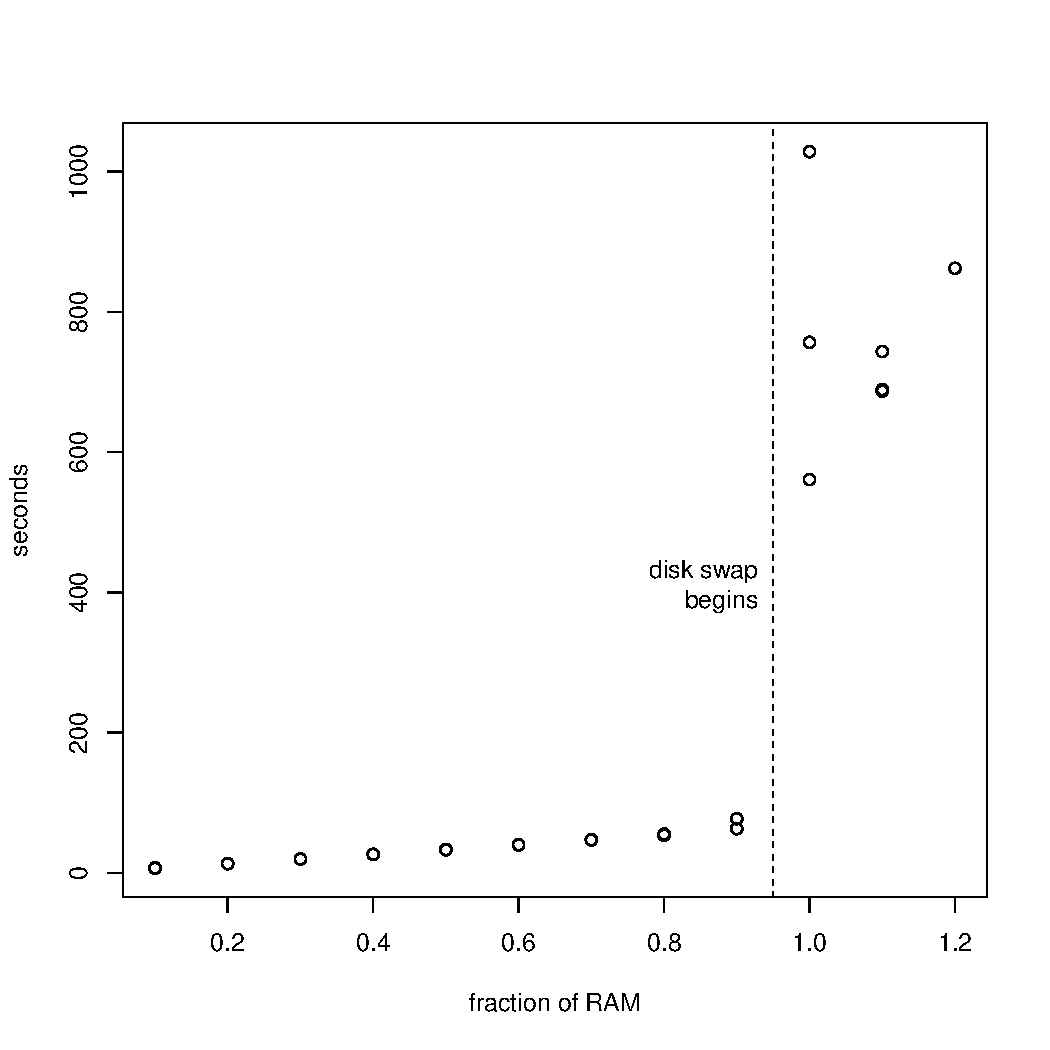
\includegraphics[width=.8\linewidth]{swap/spinning_disk_swap}
\caption{Performance is reasonable while data fits in memory.}
\label{fig:spinning_disk_swap}
\end{figure}

Compilation can alleviate this issue, but it can't resolve it, since it
can't give the system more memory. It may be able to help reduce the
creation of large intermediate data objects.


\section{Extra examples}

Andrew Latimer's regression across pixels of images over time to predict
tree death. 400 images each of which is 50 million pixels?

Climate Corporation smoothing temperatures data into different
spatiotemporal resolutions.

\section{Miscellaneous}

Here's my philosophy for software design:

\begin{itemize}
    \item Code should be as simple and straightforward. I hate code, and want as
        little of it in my codebase as possible.
    \item Fewer dependencies are better. I don't want to foist any
        particular package or way of doing things on users.
    \item Avoid choosing. If there's some way to pass things through to the
        user, ie. R's $\dots$, then use that rather than choosing for them.
\end{itemize}

\section{Scratch}

Given an exponential family with parameter $\theta$, consider evaluating
the log likelihood. An appealing property of exponential families is that
one can compute the likelihood for an iid sample by summing the
sufficient statistics $T(x_i)$.

TODO: Numerical issues with sums this large.

More concretely Ethan's likelihood for the cosmic microwave background. 
This is just one sample, but one could observe many samples.
If $\theta \in \mathbb{R}^m$ is high dimensional, then it may be
especially desirable to use many data points when computing likelihood.



